% !TeX root = RJwrapper.tex
\title{ggplot2 compatible Quantile-quantile plots in R}
\author{by Alexander Almeida, Adam Loy, Heike Hofmann}

\maketitle

\abstract{%
An abstract of less than 150 words.
}

\subsection{TODO:}\label{todo}

\begin{itemize}
\tightlist
\item
  Order of authorship?
\item
  Review Q-Q plots and P-P plots, including other arrangements, and what
  is implemented in other packages
\item
  Write about what the package implements
\item
  Give examples

  \begin{itemize}
  \tightlist
  \item
    Heike: BRFSS example
  \end{itemize}
\item
  Intro/conclusion
\item
  Abstract
\end{itemize}

\subsection{Introduction}\label{introduction}

\label{sec:introduction}

Univariate distributional assessment is a common thread throughout
statistical analyses during both the exploratory and confirmatory
stages. When we begin exploring a new data set we often consider the
distribution of individual variables before moving on to explore
multivariate relationships. After a model has been fit to a data set, we
must assess whether the distributional assumptions made were reasonable,
and if they are not we then must understand the impact this has on the
conclusions. Graphics provide arguably the most common way to carry out
these univariate assessments. While there are many graphical methods
that can be used for distribution exploration and assessment,
probability plotting is one of the most common graphical approaches
used.

Probability plotting refers to a family of methods based on the
cumulative distribution function (CDF), most notably quantile (Q-Q)
plots and probability (P-P) plots \citep{Wilk1968-ii}. In this paper, we
focus on comparing an empirical distribution to a theoretical
distribution. Let \(Y_1, \ldots, Y_n\) denote a random sample from an
unknown population, and let \(\widehat{F}_y(q)\) be the empirical
cumulative distribution obtained from the sample. Further, let \(F(q)\)
denote the CDF of a proposed dsitribution for the sample. A Q-Q plot is
constructed by plotting the quantiles of the empirical distribution,
\(q_y(p) = F_y^{-1}(p)\), against the corresponding quantiles of the
theoretical distribution, \(q(p) = F^{-1}(p)\). This constuction is
illustrated in Figure \ref{fig:qq}. A P-P plot is constructed by
plotting \(F(q)\) against \(\widehat{F}_y(q)\) for various quantiles,
\(q\). This constuction is illustrated in Figure \ref{fig:pp}.
Regardless of the plot constructed, if the two distributions are
identical, then the scatterplots will be linear with slope 1 and
intercept 0. Additionally, Q-Q plots are invariant to linear
transformations, so if two random variables differ by a linear
transformation a Q-Q plot showing draws from their distributions will
still be linear, but with a different slope and intercept, as seen in
Figure \ref{fig:qq}. P-P plots, in turn, are sensitive to linear
transformations.

\begin{Schunk}
\begin{figure}

{\centering \includegraphics[width=.45\linewidth]{qqplotr_files/figure-latex/unnamed-chunk-1-1} \includegraphics[width=.45\linewidth]{qqplotr_files/figure-latex/unnamed-chunk-1-2} 

}

\caption{\label{fig:qq}Illustrating what quantities are being plotted for Q-Q plots.}\label{fig:unnamed-chunk-1}
\end{figure}
\end{Schunk}

\begin{Schunk}
\begin{figure}

{\centering \includegraphics[width=.45\linewidth]{qqplotr_files/figure-latex/unnamed-chunk-2-1} \includegraphics[width=.45\linewidth]{qqplotr_files/figure-latex/unnamed-chunk-2-2} 

}

\caption{\label{fig:pp}Illustrating what quantities are being plotted for P-P plots.}\label{fig:unnamed-chunk-2}
\end{figure}
\end{Schunk}

While the basic form of both the Q-Q and P-P plots is a scatterplot,
additional graphical elements are often added to aid in distributional
assessment. For Q-Q plots, a reference line is often drawn through the
points \((q(.25), q_y(.25))\) and \((q(.75), q_y(.75))\). For P-P plots
a reference line with slope 1 and intercept 0 is used. In both plots,
pointwise or simultaneous confidence bands are often added around the
reference line to further aid in the visual assessment.

Innovations to Q-Q and P-P plots have also been proposed.
\citet{Loy2016-fg} discuss the creation of detrended Q-Q plots, where
the \(y\)-axis is changed to show the difference between \(q_y\) and the
reference line. Consequently, the line representing the agreement with
the theoretical distribution is the \(x\)-axis. \citet{Loy2016-fg} find
that detrended Q-Q plots are more powerful than other designs, so long
at the \(y\)-axis limits are set so that the aspect ratio is kept the
same as in the traditional Q-Q plot. In reliability and survival
analysis, probability plots often refer to a hybrid probability plot,
there the CDF of the proposed theoretical distribution is plotted
against the empirical order statistics, and transformations are applied
to each axis to linearize the CDF \citep[cf.][chapter 6]{Meeker1998}.
This hybrid probability plot is invariant to linear transformations.

\begin{Schunk}
\begin{figure}

{\centering \includegraphics[width=.31\linewidth]{qqplotr_files/figure-latex/unnamed-chunk-3-1} \includegraphics[width=.31\linewidth]{qqplotr_files/figure-latex/unnamed-chunk-3-2} \includegraphics[width=.31\linewidth]{qqplotr_files/figure-latex/unnamed-chunk-3-3} 

}

\caption{\label{fig:pp-designs}Illustrating different designs of probability plots.}\label{fig:unnamed-chunk-3}
\end{figure}
\end{Schunk}

Q-Q plots have been implemented in various forms in R, but none provide
a complete implementation of the probability plotting framework. Normal
quantile plots, where a sample is compared to the standard normal
distribution, are implemented using the \texttt{qqplot} and
\texttt{qqline} in \pkg{base} graphics \citep{R}. \texttt{qqmath} in
\pkg{lattice} provides a general framework for Q-Q plots, comparing a
sample to any theoretical distribution by specifying the quantile
function \citep{lattice}. \texttt{qqPlot} in the \pkg{car} package also
allows for the assessment of non-normal distribution and adds pointwise
confidence bands based on the standard errors of the order statistics or
the parametric bootstrap \citep{car}. \pkg{ggplot2} provides
\texttt{geom\_qq} and \texttt{geom\_qq\_line}, enabling the creation of
traditional Q-Q plots with a reference line, much like those created
using \texttt{qqmath}. \pkg{qqplotr} extends \pkg{ggplot2} to provide
the most complete implementation of probability plotting.

XXX \texttt{qualityTools} \cite{qualityTools}

In the remainder of this paper, we introduce the probability plotting
framework provided by \pkg{qqplotr}\ldots{} FILL THIS IN ONCE OTHER
SECTIONS ARE WRITTEN\ldots{}

TODO: FIGURE OUT WHERE TO INTRODUCE TS BANDS \citep{Aldor-Noiman2013-xw}

\subsection{\texorpdfstring{Implementing probability plots in the
\pkg{ggplot2}
framework}{Implementing probability plots in the  framework}}\label{implementing-probability-plots-in-the-framework}

With \pkg{qqplotr} we extend some of the original \pkg{ggplot2}
probability plot functionatilites by permitting the drawing of Q-Q and
P-P points, lines, and confidence bands. Our approach was to provide a
\pkg{ggplot2} layering mechanism so that for each one of those plot
elements we implemented a \pkg{ggplot2} ``stat'' (statistical
transformation). In addition, we also implemented a \pkg{ggplot2}
``geom'' (geometrical object) specifically for the confidence bands.
That geom permits a simpler way of handling graphical parameters, which
will become clearer in the \nameref{sec:examples} section.

For simplicity, the Q-Q and P-P functions will be presented separately
below.

\subsubsection{Q-Q}\label{q-q}

The Q-Q plot functions are divided into three stats:

\begin{itemize}
\item
  \texttt{stat\_qq\_point}: a modified verion of \texttt{stat\_qq} from
  \pkg{ggplot2} that plots the sample quantiles versus the theoretical
  quantiles (as in Figure \ref{fig:qq}). The novelty of this
  implementation is an option to detrend the plotted points (see
  \nameref{sec:introduction}). Moreover, all other implemented stats
  from Q-Q and P-P plots also allow the detrend adjustment.
\item
  \texttt{stat\_qq\_line}: draws a reference line based on the sample
  data quantiles, defaulting to the first and third quartiles.
\item
  \texttt{stat\_qq\_band}: draws confidence bands based on three
  methods: \emph{Normal}, \emph{Bootstrap}, and \emph{Tail-sensitive}:

  \begin{itemize}
  \tightlist
  \item
    \textbf{Normal}: constructs simultaneous confidence bands based on
    normal distribution confidence intervals;
  \item
    \textbf{Bootstrap}: creates pointwise confidence bands with
    parametric boostrap;
  \item
    \textbf{Tail-sensitive}: builds tail-sensitive confidence bands, as
    proposed by \citet{Aldor-Noiman2013-xw}.
  \end{itemize}
\end{itemize}

\subsubsection{P-P}\label{p-p}

The P-P plot functions are also divided into three plot elements:

\begin{itemize}
\item
  \texttt{stat\_pp\_point}: plots cumulative probabilities versus
  probability points (as in Figure \ref{fig:pp}).
\item
  \texttt{stat\_pp\_line}: draws a reference identity line (slope 1 and
  intercept 0).
\item
  \texttt{stat\_pp\_band}: draws confidence bands. For now, only the
  bootstrap version (\texttt{"bs"}) is available.
\end{itemize}

TODO: TALK MORE IN-DEPTH ABOUT THE FUNCTIONS' PARAMETERS.

\subsection{Examples}\label{examples}

\label{sec:examples}

In this section, we demonstrate the capabilities of the \textbf{qqplotr}
package.

\begin{Schunk}
\begin{Sinput}
library(qqplotr)
\end{Sinput}
\end{Schunk}

\subsubsection{BRFSS example}\label{brfss-example}

The Center for Disease Control and Prevention runs an annual telephone
survey, the Behavioral Risk Factor Surveillance System (BRFSS), to keep
track of the US populations' `health-related risk behaviors, chronic
health conditions, and use of preventive services'.\\
Close to half a million interviews are conducted each year. Here, we are
focussing on the 2012 responses for Iowa. 7166 responses were gathered
across 359 questions and derived variables. Among these, are people's
height and weight, which we are going to assess in more detail.

Figure \ref{fig:heights} shows two Q-Q plots side by side. For each of
the plots, a sample of 200 men and 200 women is drawn from the overall
number of responses. On the left hand side, individuals' heights are
plotted in a Q-Q plot comparing raw heights to a normal distribution. We
see that the distributions for both men and women (colour) is showing
horizontal steps: this indicates that the distributional assessement is
heavily dominated by the discreteness in the data, as most survey
participants responded to the question of their height to the closest
inch. On the right hand side of figure \ref{fig:heights}, we use
jittering; this means that we add a random number generated from a
random uniform distribution on \(\pm 0.5\) inch to the reported height.
By this mean we extinguish any effect that discreteness might have on
the distribution. This brings the observed distribution much closer to a
normal distribution. Note that separate normal distributions were fitted
for each gender, not surprisingly, the resulting distributions have
different means (women are on average 6 inch shorter than men in this
dataset). Interestingly, the slope of the two genders is similar,
indicating that the same scale parameter fits both genders'
distributions (the standard deviation of height in the data set is 2.97
inch for men and 2.91 inch for women).

\begin{Schunk}
\begin{figure}

{\centering 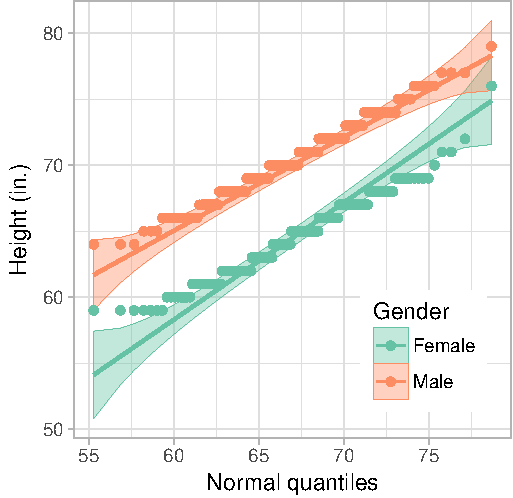
\includegraphics[width=\textwidth]{qqplotr_files/figure-latex/heights-1} 

}

\caption[Sample (200 men and 200 women) of raw heights (left) and jittered heights (right)]{Sample (200 men and 200 women) of raw heights (left) and jittered heights (right). The distribution on the left is dominated by the discreteness of the data. On the right we see that except for some outliers an assumption of normality for people's height is not completely absurd.}\label{fig:heights}
\end{figure}
\end{Schunk}

Unlike respondents' heights, their weigths do not seem to be normally
distributed. Figure \ref{fig:weights} shows again two Q-Q plots. The Q-Q
plot on the left uses raw weights and compares to a normal distribution.
From the curved points we see that tails of the observed distribution
are heavier than expected under a normal distribution. On the right,
weights are log-transformed. We see that a normal distribution for each
of the genders shows --with the exceptions of a few extreme outliers-- a
reasonable fit.

\begin{Schunk}
\begin{figure}

{\centering 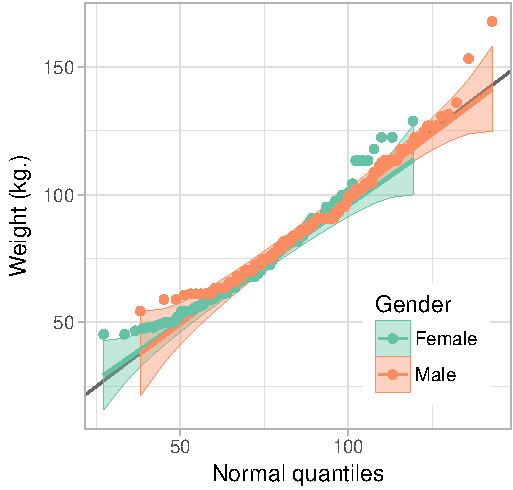
\includegraphics[width=\textwidth]{qqplotr_files/figure-latex/weights-1} 

}

\caption[Sample (200 men and 200 women) of weights]{Sample (200 men and 200 women) of weights. Unlike people's height, weight seems to be heavily right skewed with some additional outliers on the extreme left. (left plot), on the right, weight was log-transfomed before its distribution is compared to a theoretical normal. }\label{fig:weights}
\end{figure}
\end{Schunk}

Instead of transforming the observed values, we can change the
theoretical distribution against which we compare. Figure
\ref{fig:weights-log} shows two Q-Q plots where a a log-normal
distribution is choses as the theoretical distribution. On the left, we
compare against a log-normal distribution with mean 4.389 and standard
deviation 0.223 (the log-transformed averages of average weight and
standard deviation in Iowa's population). Again, the fits seem
reasonable. On the right, parameters for the log-normal distribution are
fit separately. The fits are slightly different from

\begin{Schunk}
\begin{figure}

{\centering 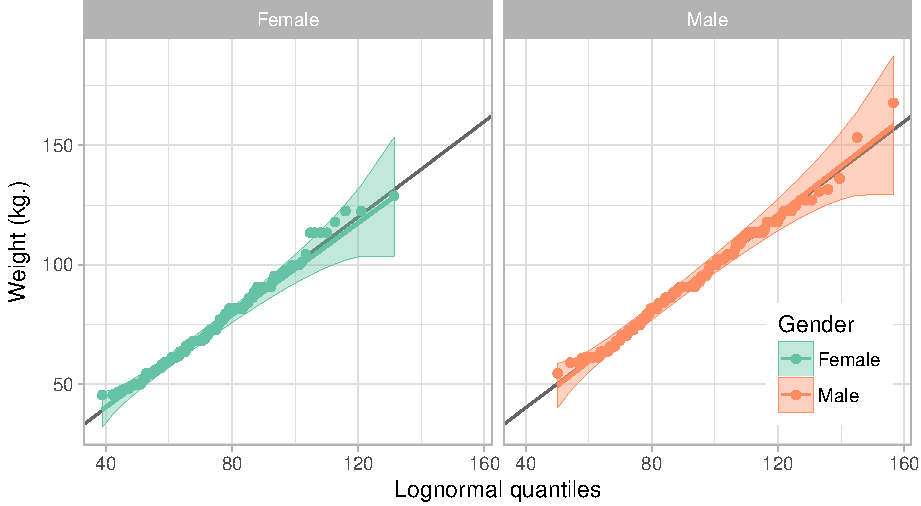
\includegraphics[width=\textwidth]{qqplotr_files/figure-latex/weights-log-1} 

}

\caption[Sample (200 men and 200 women) of weights]{Sample (200 men and 200 women) of weights. On the left, the theoretical distribution  is changed to a log normal. On the right, we additionally estimate shift and scale parameters for each of the genders separately before comparing distributions to a log-normal. XXX need to fix alpha}\label{fig:weights-log}
\end{figure}
\end{Schunk}

\begin{table}

\caption{\label{tab:table}this table is just for us at the moment}
\centering
\begin{tabular}[t]{r|r|r|r|r}
\hline
SEX & mean\_wt & mean\_log\_wt & sd\_wt & sd\_log\_wt\\
\hline
1 & 91.50342 & 4.495766 & 19.22981 & 0.2011216\\
\hline
2 & 74.37085 & 4.282780 & 17.90126 & 0.2254663\\
\hline
\end{tabular}
\end{table}

\subsubsection{Using a non-standard
distribution}\label{using-a-non-standard-distribution}

ADAM: PULL DATA OFF EXTERNAL HARD DRIVE, EXPLAIN THE EXAMPLE\ldots{}

The ``standard'' distributions provided in \texttt{pkg\{stats\}} do not
include a left-skewed distribution, which is clearly needed to model the
long jump heights. To handle this type of situation, \pkg{qqplotr} let's
users create probability plots for all of the distributions defined in
the \pkg{stats} package as well as other sources, so long as the
distributions are defined following the conventions laid out in the
\pkg{stats} package. Specfically, for some distribution there must be
density/mass (\texttt{d} prefix), CDF (\texttt{p} prefix), quantile
(\texttt{q} prefix), and simulation (\texttt{r} prefix) functions.

To illustrate this process we will consider the smallest exreme value
(SEV) distribution. This is a left-skewed distribution, which is a key
feature needed in order to model the long jump results. Below, we define
the suite of distribution functions needed to utilize the SEV
distribution.

\begin{Schunk}
\begin{Sinput}
# CDF
psev <- function(q, mu, sigma) {
    z <- (q - mu) / sigma
    1 - exp(-exp(z))
}

# PDF
dsev <- function(x, mu, sigma) {
  z <- (x - mu) / sigma
  (1 / sigma) * exp(z - exp(z))
}

# Quantile function
qsev <- function(p, mu, sigma) {
  mu + log(-log(1 - p)) * sigma
}

# Simulation function
rsev <- function(n, mu, sigma) {
  qsev(runif(n), mu, sigma)
}
\end{Sinput}
\end{Schunk}

\subsection{Summary}\label{summary}

Write this section once the rest of the paper is done.

\bibliography{RJreferences}

\subsection{Acknowledgements}\label{acknowledgements}

Mention GSoC here\ldots{}

\address{%
Alexander Almeida\\
Affiliation\\
line 1\\ line 2\\
}
\href{mailto:author1@work}{\nolinkurl{author1@work}}

\address{%
Adam Loy\\
Affiliation\\
line 1\\ line 2\\
}
\href{mailto:author2@work}{\nolinkurl{author2@work}}

\address{%
Heike Hofmann\\
Iowa State University\\
Department of Statistics\\ Ames, IA 50011-1210\\
}
\href{mailto:hofmann@iastate.edu}{\nolinkurl{hofmann@iastate.edu}}

